\clearpage
\begin{explanationbox}
\textbf{\textcolor{CExplanation}{一、先看图：为什么是“水平移动”？}}
\par\noindent\begin{minipage}{\linewidth}
\begin{center}
\begingroup
\def\Cmode{1}
% Exact model: p=2, A=(1,-2), B=(4,4), M=(-2,1), N=(5/2,1).
\begin{tikzpicture}[x=1.15cm,y=0.85cm,>=stealth,font=\small]
\path[use as bounding box] (-3.1,-3.5) rectangle (6.1,5.2);
\draw[->,gray] (-2.9,0)--(5.7,0) node[right] {$x$};
\draw[->,gray] (0,-2.8)--(0,4.9) node[above] {$y$};
\node[below left] at (0,0) {$O$};
\draw[blue,thick,domain=-2.5:4.5,samples=100] plot ({\x*\x/4},\x);
\node[blue,right] at (5.1,4.2) {$y^2=4x$};
\draw[orange,thick] (-2.6,1.6)--(1.6,-2.6);
\draw[orange,thick] (-2.6,.7)--(5,4.5);
\draw[gray,thick] (1,-2)--(4,4);
\draw[red,very thick] (-2,1)--(2.5,1);
\ifnum\Cmode=1
  \draw[dashed,gray] (1,-2)--(-.55,-2) (4,4)--(-.55,4);
  \draw[<->,blue] (-.55,-2)--(-.55,1) node[midway,left,fill=white,inner sep=2pt] {$3$};
  \draw[<->,blue] (-.55,1)--(-.55,4) node[midway,left,fill=white,inner sep=2pt] {$3$};
  \fill[red] (0,1) circle (2pt) node[above left=2pt] {$H$};
\fi
\ifnum\Cmode=2
  \draw[dashed,blue] (1,-2)--(4,-2)--(4,4);
  \node[below,blue] at (2.5,-2.7) {$\Delta x=3$};
  \node[right,blue,fill=white,inner sep=2pt] at (4,-.6) {$\Delta y=6$};
  \node[fill=white,inner sep=3pt] at (2.8,4.85) {$AB:\ x=\tfrac12y+2,\quad pt=1$};
\fi
\ifnum\Cmode=3
  \node[fill=white,inner sep=3pt] at (2.7,4.85) {$AB:\ y=2(x-2)$};
  \node[anchor=west,fill=white,inner sep=3pt] at (3.4,2) {$y_1=-2,\ y_2=4$};
\fi
\ifnum\Cmode=4
  \draw[dashed,red] (-2,1)--(-2,-.7) (2.5,1)--(2.5,-.7);
  \draw[<->,red] (-2,-.6)--(2.5,-.6) node[pos=1,below right,fill=white,inner sep=3pt] {$x_N-x_M=\tfrac92>0$};
\fi
\fill (1,-2) circle (2pt) node[right=10pt] {$A(1,-2)$};
\fill (4,4) circle (2pt) node[above left] {$B(4,4)$};
\fill[red] (-2,1) circle (2pt) node[below left] {$M(-2,1)$};
\fill[red] (2.5,1) circle (2pt) node[below right,fill=white,inner sep=2pt] {$N(\tfrac52,1)$};
\ifnum\Cmode=0
  \node[red,above,fill=white,inner sep=3pt] at (.6,1) {$y_M=y_N=1$};
\fi
\end{tikzpicture}

\endgroup


图取 $y_1=-2,y_2=4$，平均高度为 $1$；$H,M,N$ 同在高度 $1$ 上。
\end{center}
\end{minipage}\par

\medskip
\textbf{\textcolor{CExplanation}{二、从“中点”理解结论}}
图中 $A,B$ 在 $y$ 轴上的投影高度分别为 $-2,4$，$H(0,1)$ 恰在两高度的正中间。
对一般的 $y_1,y_2$，这一平均高度为 $(y_1+y_2)/2$；结论说明 $M,N$ 也在此高度上。

\medskip
\textbf{\textcolor{CExplanation}{三、为什么切线方程适用于顶点？}}
在 $y^2=2px$ 上取 $T(x_0,y_0)$，由于 $y_0^2=2px_0$，直线
\[
 yy_0=p(x+x_0)
\]
与抛物线联立时，把 $x=yy_0/p-x_0$ 代入 $y^2=2px$：
\[
 y^2=2yy_0-2px_0=2yy_0-y_0^2,
 \quad\text{即}\quad (y-y_0)^2=0.
\]
它只在 $T$ 处与抛物线相遇，所以就是 $T$ 处的切线。
\textbf{这段验证只用平方差、完全平方和方程，不用求导；}
即使 $T$ 是顶点 $O(0,0)$，公式也给出 $x=0$，仍然成立。

\medskip
\textbf{\textcolor{CExplanation}{四、最关键的一步为什么会出现平均数？}}
两条切线相减时，交点的横坐标 $x_M$ 被消去，得到
\[
(y_1-y_2)y_M=p(x_1-x_2).
\]
再利用 $x_i=y_i^2/(2p)$，右侧成为
\[
 p(x_1-x_2)=\frac{y_1^2-y_2^2}{2}
 =\frac{(y_1-y_2)(y_1+y_2)}2.
\]
消去不为零的 $y_1-y_2$，便得到 $y_M=(y_1+y_2)/2$。
\textbf{记住几何意义：两个切点的“高度平均值”，正好是切线交点的高度。}

\medskip
\textbf{\textcolor{CExplanation}{五、进一步看水平距离}}
两个点虽处在同一高度，但并不重合：
\[
x_N-x_M=\frac{(y_1-y_2)^2}{4p}.
\]
因为 $A\ne B$ 蕴含 $y_1\ne y_2$，所以分子严格大于 $0$。
这说明 $M$ 与 $N$ 在水平方向上\textbf{必有间隔}，而且间隔大小是
\[
|MN|=\frac{(y_1-y_2)^2}{4|p|}.
\]
从图形上看，两切点的纵坐标差越大，$MN$ 越长（在 $p$ 固定时）；
$p$ 的正负只决定向左还是向右。

\medskip
\textbf{\textcolor{CExplanation}{六、考场识别信号}}
\begin{itemize}[leftmargin=*,itemsep=0.35em,topsep=0.3em]
\item \textbf{出现“两点处的切线相交＋弦中点”：}先确定一个坐标相同，不必立刻解完整方程组。
\item \textbf{已知弦方程 $x=ty+q$：}可直接得到 $y_M=y_N=pt$；这里的 $t$ 是 $x$ 随 $y$ 的变化比值，不是通常的 $\Delta y/\Delta x$ 斜率。
\item \textbf{两切点纵坐标互为相反数：}连线 $MN$ 就在 $x$ 轴上。
\item \textbf{$x^2=2py$：}交换横、纵坐标，结论变成 $x_M=x_N$，$MN$ 竖直。
\end{itemize}
\end{explanationbox}
